\section{Variabili aleatorie}
Introduciamo ora uno strumento cardine dello studio della probabilità: la \emph{variabile aleatoria}, nome che denota una quantità ignota a priori, il cui valore dipende dall'esito di un esperimento aleatorio.
Essa associa gli esiti elementari su un dominio $\Omega$, anche non numerico, a valori reali su un codominio $F$, trasformando gli eventi sul dominio in eventi sul codominio.
L'enorme utilità di questo strumento risiede proprio nel permettere l'applicazione della teoria su $\RR$ precedentemente introdotta, spostando l'attenzione da un dominio generico a un codominio numerico, molto più facile da analizzare.
Agli eventi sul codominio, similmente a quanto visto per il dominio, è associata una probabilità, detta \emph{legge} della variabile aleatoria, da cui discende la nozione di \emph{uguaglianza quasi certa} tra variabili aleatorie.
Sarà inoltre analizzato il concetto di \emph{misurabilità}, proprio delle variabili aleatorie, e le relative proprietà.

\subsection{Definizione}

\begin{defn}
   Data una funzione $X: \Omega \to F$ e un insieme $B \subseteq F$, si dice \textbf{controimmagine} di $B$ l'insieme
   $X^{-1}(B) = (X \in B) \coloneqq \{ \omega \in \Omega: X(\omega) \in B\} \subseteq \Omega$.
\end{defn}

\begin{figure}[H]
  \centering
  \def\firstcircle{(0,0) circle (1.2cm)}
  \def\drect {(-1.5, -1.5) rectangle (1.5, 1.5)}
  \begin{tikzpicture}
    \begin{scope}
      \fill[lightgray] \firstcircle;
      \draw \drect node[below left] {\large $\Omega$};
      \draw \firstcircle node {\large $(X \in B)$};
    \end{scope}

    \draw[->, line width=0.30mm] (1.8,0) node[above,xshift=1.2cm] {\Large $X$} -- (4.2,0);

    \begin{scope}[shift={(6cm,0cm)}]
      \fill[lightgray] \firstcircle;
      \draw \drect node[below left] {\large $F$};
      \draw \firstcircle node {\large $B$};
    \end{scope}
  \end{tikzpicture}
  \caption{immagine e controimmagine di una VA}
\end{figure}

\smallskip
\begin{defn}
  \index{variabile aleatoria}
  Dati gli spazi misurabili $(\Omega, \Ac)$ e $(F, \Fc)$,
  una funzione $X: \Omega \to F$ si dice \textbf{funzione misurabile}
  o \textbf{variabile aleatoria} (abbreviato in \textbf{VA}) se:
  \begin{center}
  	$(X \in B) \in \Ac \enspace \forall B \in \Fc$
  \end{center}
\end{defn}
Talvolta useremo la notazione sintetica $X: \Dom \to (F, \Fc)$ per indicare che $X$ è una variabile aleatoria (o una funzione) che ha dominio $\Omega$ e codominio $F$, che a $\Omega$ è associato lo spazio di probabilità $\Dom$ e che a $F$ è associato lo spazio misurabile $(F, \Fc)$.

\smallskip
\begin{defn}
  \index{spazio!degli stati}
  L'insieme $F$ che contiene tutti
  i possibili valori della VA si dice \textbf{spazio degli stati}.
\end{defn}

\textit{Proprietà della controimmagine:}
\begin{itemize}
  \item $(X \in B^C) = X^{-1}(B^C) = (X^{-1}(B))^C = (X \in B)^C = (X \not\in B)$
  \item $(X \in \bigcup\limits_n B_n) = \bigcup\limits_n \ (X \in B_n)$
  \item $(X \in \bigcap\limits_n B_n) = \bigcap\limits_n \ (X \in B_n)$
\end{itemize}

\medskip
\begin{ese}
  Definiti $\Omega = \{ 1, \dots, 6 \}^2$, $\Ac = 2^\Omega$, $F = \RR$, $\Fc = \Bc$, $X: \Omega \to \RR$ e $X(\omega) = \omega_1 + \omega_2$ la variabile aleatoria associa ad un evento nella $\Fc$ (es. \textit{la somma dei due dadi dà 3}) un evento nella $\Ac$.

In questo caso si consideri l'evento $B = \{ 3 \}$: allora $(X \in B) = \{ (1, 2), (2, 1) \} \in \Ac$.\\
Inoltre $\operatorname{im}(X) = (2, \dots, 12) $, $ \; \#\operatorname{im}(X) = 11 \le \#\operatorname{im}(\Omega) = 36$, infatti
ogni evento elementare può avere al massimo un esito.
  \begin{figure}[H]
    \centering
    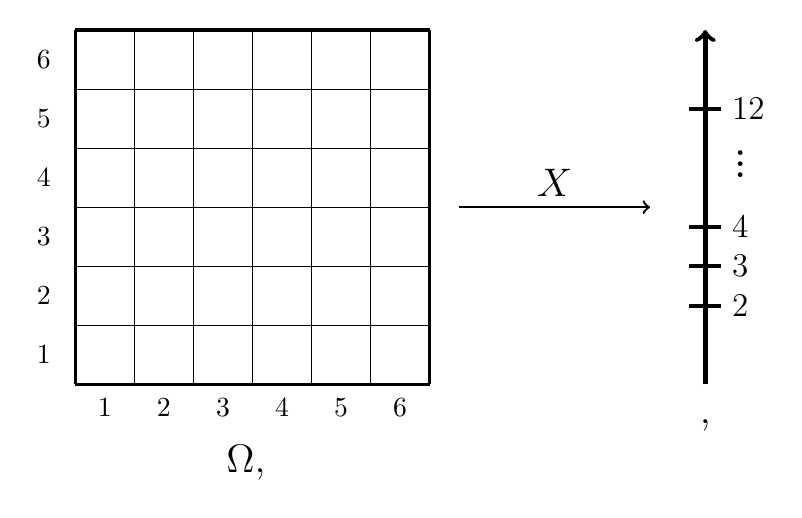
\begin{tikzpicture}
      \begin{scope}
          \draw[scale=0.75] (0, 0) grid (6,6);
          \draw[very thick, scale=4.5] (0, 0) grid (1, 1);
          %Verticali
          \node at (-0.4, 0.375) {$1$};
          \node at (-0.4, 1.125) {$2$};
          \node at (-0.4, 1.875) {$3$};
          \node at (-0.4, 2.625) {$4$};
          \node at (-0.4, 3.375) {$5$};
          \node at (-0.4, 4.125) {$6$};
          %Orizzontali
          \node at (0.375, -0.3) {$1$};
          \node at (1.125, -0.3) {$2$};
          \node at (1.875, -0.3) {$3$};
          \node at (2.625, -0.3) {$4$};
          \node at (3.375, -0.3) {$5$};
          \node at (4.125, -0.3) {$6$};
          \node[anchor=center] at (2.25, -1) {\Large $\Omega, \ \Ac$};
          %Frecce
          \draw[->, line width=0.30mm] (4.875,2.25) node[above,xshift=1.2125cm] {\Large $X$} -- (7.3,2.25);
          \draw[->, line width=0.60mm] (8,0) node[below, yshift=-.3cm] {\Large $\RR, \Bc$} -- (8,4.5);
          %Tacchette
          \draw[line width=0.50mm] (8.2,1) node[right] {\large $2$} -- (7.8, 1);
          \draw[line width=0.50mm] (8.2,1.5) node[right] {\large $3$} -- (7.8, 1.5);
          \draw[line width=0.50mm] (8.2,2) node[right] {\large $4$} -- (7.8, 2);
          \node at (8.45, 2.9) {\huge $\vdots$};
          \draw[line width=0.50mm] (8.2,3.5) node[right] {\large $12$} -- (7.8, 3.5);
        \end{scope}
      \end{tikzpicture}
    \caption{somma del lancio di due dadi}
  \end{figure}
\end{ese}

\bigskip

\begin{ese}
  Definita %$\Omega = \RR$, $\Ac = \Bc$, $F = \RR$, $\Fc = \Bc$, $\PP = \Ec(\lambda)$, $X:\RR \to \RR$ e $X(\omega) = \ceil{\omega}$
  la funzione $X: (\RR, \Bc, \PP) \to (\RR, \Bc)$, con $X(\omega) = \ceil\omega$ e $\PP = \Ec(\lambda)$,
  si può affermare che $\operatorname{im}(X) = \ZZ$ e $(X \in B) \in \Ac = \Bc \ \ \forall B \in \Fc$. \\
  $X$ è effettivamente una VA poiché $(X \in B)$ è un'unione al più numerabile di intervalli
  del tipo $(k, k+1] \ (k \in \ZZ)$, cioè $(X \in B) \in \Bc$.
  \begin{figure}[H]
    \centering
    \begin{tikzpicture}
      \begin{axis}[
          axis lines = middle,
          ylabel = $X(\omega)$,
          xlabel = $\omega$,
          width=0.8\textwidth,
          height=0.5\textwidth
      ]

      \draw [line width=0.3mm] (axis cs:-2,-1) -- (axis cs:-1, -1);
      \draw [line width=0.3mm] (axis cs:-1,0) -- (axis cs:0,0);
      \draw [line width=0.3mm] (axis cs:0,1) -- (axis cs:1,1);
      \draw [line width=0.3mm] (axis cs:1,2) -- (axis cs:2,2);
      \draw [line width=0.3mm] (axis cs:2,3) -- (axis cs:3,3);

      \addplot [only marks, mark=*] table {
      -1 -1
      0 0
      1 1
      2 2
      };

      \addplot [draw=none, forget plot] coordinates {(-1.5,-1.2)};
      \addplot [draw=none, forget plot] coordinates {(2.5, 3.2)};

      \addplot [draw=none, forget plot] coordinates {(0,-1.2)};
      \addplot [draw=none, forget plot] coordinates {(0,3.2)};

      \end{axis}
    \end{tikzpicture}
    \caption{rappresentazione di $X(\omega) = \ceil{\omega}$}
  \end{figure}
\end{ese}

\bigskip

\begin{ese}
  Definita %$\Omega = \RR$, $\Ac = \Bc$, $F = \RR$, $\Fc = \Bc$, $\PP = \Ec(\lambda)$, $X: \RR \to \RR$ e $X(\omega) = \omega$
  la funzione $X: (\RR, \Bc, \PP) \to (\RR, \Bc)$, con $X(\omega) = \omega$ e $\PP = \Ec(\lambda)$,
  allora si può affermare che $\operatorname{im}(X) = \RR$. Le controimmagini coincidono con l'insieme
  di partenza, dunque $X$ è una variabile aleatoria.
\end{ese}

\bigskip
\begin{teo}
  Siano $(\Omega, \Ac)$ e $(F, \Fc)$ spazi misurabili generici,
  $X: \Omega \to F$ una funzione, e $\Cc \subseteq \Fc$ tale che
  $\sigma(\Cc) = \Fc$. Allora:
  $$(X \in B) \in \Ac \enspace \forall B \in \Fc \enspace
    \iff \enspace (X \in B) \in \Ac \enspace \forall B \in \Cc$$
\end{teo}
In altre parole, la misurabilità su un insieme coincide con la misurabilità su un insieme più piccolo che genera l'altro insieme.

\begin{dimo}
  \textbf{($\implies$)}: ovvia. \\
  \textbf{($\impliedby$)}:
  ponendo $\Dc = \{ B \in \Fc: (X \in B) \in \Ac \}$ si ha che $\Cc \subseteq \Dc \subseteq \Fc$ e che $\Dc$ è una $\sigma\text{-algebra}$ poiché unioni, intersezioni, e complementazioni commutano con le controimmagini, infatti:
  \begin{align*}
    B \in \Dc &\implies (X \in B) \in \Ac
    \implies (X \in B)^C \in \Ac\\
    &\implies (X \in B^C) \in \Ac
    \implies B^C \in \Dc
  \end{align*}

  Dalla prima relazione ($\Cc \subseteq \Dc \subseteq \Fc$)
  otteniamo $\sigma(\Cc) \subseteq\sigma(\Dc) \subseteq \sigma(\Fc)$,
  da cui $\Fc \subseteq\Dc \subseteq \Fc$.
  Allora $\Dc = \Fc$, cioè tutti gli elementi $B$ di $\Fc$
  sono tali per cui $(X \in B) \in \Ac$, da cui la tesi. \qedhere

\end{dimo}

\lezione{8}{24.03.17}
\needspace{8\baselineskip}
\subsection{Criteri di misurabilità}
\begin{defn}
  \index{misurabilità}
  \index{funzione!misurabile}
  Siano $(E, \Ec), (F, \Fc)$ spazi misurabili. \\
  Una funzione $X: E \to F$ è detta \textbf{misurabile} se $X^{-1}(B) \in \Ec \quad \forall B \in \Fc$, oppure $X^{-1}(\Fc) \subseteq \Ec$.
\end{defn}
\begin{nb}
  Quando $(E,\Ec)=(\Omega, \Ac)$, la funzione misurabile $X$ è una variabile aleatoria.
\end{nb}

\medskip
\begin{teob}[\JPTh{8.1}]
  Siano $(E, \Ec), (F, \Fc)$ spazi misurabili, $X: E \to F$, e $\Cc \in \Fc$ tale che $\sigma(\Cc) = \Fc$. Allora:
  $$X \text{ misurabile} \iff X^{-1}(\Cc) \subseteq \Ec$$
\end{teob}
\medskip
\begin{coro}
  $(\Omega, \Ac), (\RR, \Bc)$ spazi misurabili, $X:\Omega \to \RR$, $ \; X_n:\Omega \to \RR, \ n \in \NN$
  \begin{enumerate}
    \item X è VA misurabile:
    \begin{enumerate}
      \item $\iff$ $(X \leq t) \in \Ac \quad \forall t \in \RR$
      \item $\iff$ $(X < t) \in \Ac \quad \forall t \in \RR$
    \end{enumerate}
    \item $X_n$ misurabile $\forall n$ $\implies$ sono VA:
    \begin{enumerate}
      \item $\sup\limits_n X_n$
      \item $\inf\limits_n X_n$
      \item $\limsup\limits_n X_n$
      \item $\liminf\limits_n X_n$
    \end{enumerate}
    \item $X_n$ VA misurabile $\forall n$, $X_n \underset{n}{\to} X$ puntualmente $\implies X$ VA misurabile.\\*
      Questo ci consente di lavorare con le variabili aleatorie comodamente su $\RR$ perché se $X_n(\omega) \to X(\omega) \quad \forall \omega \in \RR$ è sufficiente che il codominio sia $\RR$, senza considerare il dominio $\Omega$.
  \end{enumerate}
\end{coro}

\begin{dimo}
  Viene dimostrato solo il corollario, non il teorema.
  \begin{enumerate}
    \item
     ($\implies$) è ovvia per entrambe, dimostriamo ($\impliedby$) per (a) e (b):
    \begin{enumerate}
      \item
        Definiamo la semiretta $(-\infty, t]$ come $\Cc$:
        $$F = \RR, \ \Fc  = \Bc, \ \Cc = \{(-\infty, t], \ t \in \RR\}, \ \sigma(\Cc) = \Bc$$
        Quindi se $(X \leq t) \in \Ac \quad \forall t \in \RR \implies X$ è misurabile.
      \item
        Come sopra, definiamo la semiretta $(-\infty, t)$ come $\Cc_0$:
        $$F = \RR, \ \Fc  = \Bc, \ \Cc_0 = \{(-\infty, t), \ t \in \RR\}$$
        Possiamo affermare che $\sigma(\Cc_0) = \Bc$ costruendo una serie $\left(-\infty, t + \frac{1}{n}\right)$:
        $$\bigcap\limits_{n = 1}^{{+\infty}} \left(-\infty, t + \frac{1}{n}\right) = (-\infty, t]$$
        In questo modo si ha che $\Cc \subseteq \Cc_0$ e di conseguenza:
        $$\Bc = \sigma(\Cc) \subseteq \sigma(\Cc_0) \subseteq \Bc$$
    \end{enumerate}
    \item
    \begin{enumerate}
      \item Essendo $X$ misurabile $\{X_n \leq t\} \in \Ac$, quindi:
        $$\left\{\sup\limits_n (X_n) \leq t\right\} = \left\{\bigcap\limits_n (X_n \leq t)\right\}$$
        Essendo $X_n$ VA, si sfrutta il punto (1), ovvero $(X_n \leq t) \in \Ac$. Intersecando si può affermare che:
        $$\bigcap\limits_n (X_n \leq t) \in \Ac$$
        Servendosi di nuovo del punto (1) si mostra che $\sup\limits_n (X_n)$ è una VA.
      \item La dimostrazione di $\inf\limits_n X_n$ sarà affrontata più nel dettaglio:

        Si può definire un $\omega$ nel codominio per mostrare che è presente anche nel dominio:
        $$\omega \in \{\inf\limits_n (X_n < t)\} = \bigcup\limits_n (X_n < t), \ (X_n < t) \in \Ac$$
        Per dimostrare la prima uguaglianza si può passare per le esistenze:
        $$\omega \in \{\inf\limits_n (X_n \leq t)\} \iff \{\inf\limits_n X_n\} \leq t$$
        Essendo $\inf\limits_n X_n < t$, allora:
        \begin{align*}
          \exists n_0 \text{ tale che } X_{n_0}(\omega) < t &\iff \exists n_0 \text{ tale che } \omega \in (X_{n_0} < t) \\
          &\iff \omega \in \bigcup\limits_n (X_n < t)
        \end{align*}
        Questo ragionamento è valido per ogni $t$.
      \item $\limsup\limits_n X_n = \inf\limits_n \left(\sup\limits_{k>n} X_k \right)$: sup è misurabile per (a) e inf per (b)
      \item $\liminf\limits_n X_n = \sup\limits_n \left(\inf\limits_{k>n} X_k \right)$: sup è misurabile per (a) e inf per (b)
    \end{enumerate}
    \item $\lim\limits_n X_n = \limsup\limits_n X_n$ se $X_n$ converge puntualmente. Per la proprietà (2c) questo è misurabile. \qedhere
  \end{enumerate}
\end{dimo}

\bigskip
\begin{ese}[controimmagine di una parabola]
  Dati $\Omega = F = \RR$, $\Ac = \Fc = \Bc$, $\PP = \Ec(\lambda)$, $X(\omega) = \omega^2$ possiamo affermare che $X$ è misurabile\footnote{Spoilerone: dimostreremo che tutte le funzioni continue tra boreliani sono misurabili} se e solo se $(X \leq t) \in \Bc \ \ \forall t$, ovvero per una parabola del tipo:
  $$(X \leq t) = \begin{cases} \varnothing & t<0\\ [-\sqrt{t}, \sqrt{t}] & t\geq 0 \end{cases} \quad \in \Bc \quad \forall t$$
  In entrambi i casi la controimmagine appartiene a $\Bc$:
\begin{figure}[H]
  \centering
  \begin{tikzpicture}
  \begin{axis}[
      axis lines = middle,
      xlabel = $x$,
      ylabel = {$f(x)$},
      width=0.55\textwidth,
      yticklabels={,,},
      xticklabels={,,}
  ]
  \addplot [draw=none, forget plot] coordinates {(0,2)} node[above right] {$t>0$};
  \addplot [draw=none, forget plot] coordinates {(1.414,0)} node[below] {$\sqrt{t}$};
  \addplot [draw=none, forget plot] coordinates {(-1.414,0)} node[below, xshift=-0.1cm] {$-\sqrt{t}$};
  \draw [-|, line width=0.50mm] (axis cs:0,-5) -- (axis cs:0,2.04);
  \draw [line width=0.2mm, dashed] (axis cs:-1.414,0) -- (axis cs:-1.414,2) -- (axis cs:1.414,2) -- (axis cs:1.414,0);
  \draw [-, line width=0.2mm, decorate,decoration={snake,amplitude=.4mm,segment length=2mm,post length=0mm}] (axis cs:-1.414,0) -- (axis cs:1.414,0);
  \addplot [
      domain=-2:2,
      samples=100,
      color=lightblue,
      line width=0.3mm
      ]
      {x^2};
  \addplot [draw=none, forget plot] coordinates {(0,-3)};
  \end{axis}
  \end{tikzpicture}
  \hskip 5pt
  \begin{tikzpicture}
  \begin{axis}[
      axis lines = middle,
      xlabel = $x$,
      ylabel = {$f(x)$},
      width=0.55\textwidth,
      yticklabels={,,},
      xticklabels={,,}
  ]
  \addplot [draw=none, forget plot] coordinates {(0,-1)} node[right, xshift=0.15cm] {$t<0$};
  \draw [-|, line width=0.50mm] (axis cs:0,-5) -- (axis cs:0,-1);
  \addplot [
      domain=-2:2,
      samples=100,
      color=lightblue,
      line width=0.3mm
      ]
      {x^2};
  \addplot [draw=none, forget plot] coordinates {(0,-3)};
  \end{axis}
  \end{tikzpicture}
  \label{controimmagine-parabola}
  \caption{controimmagine di una parabola}
\end{figure}
\end{ese}

\subsection{Proprietà delle funzioni misurabili}
\begin{teo}[composizione di funzioni misurabili \JPTh{8.2}]\label{teo-comp-misurabili}
  \index{composizione di funzioni misurabili}
  $(\Omega, \Ac), (F, \Fc), (G, \Gc)$ spazi misurabili, $X:\Omega \to F$, $h:F \to G$. Allora:
  $$X \text{ e } h \text{ misurabili}\implies Y = h \circ X = h(X):\Omega \to G \text{ misurabile}$$
\end{teo}
\begin{dimo}
  Si sceglie $B$ nella $\sigma$-algebra finale $\Gc$, ovvero $B \in \Gc$. La controimmagine è: %l a s i g m a a l g e b r a f i n a l e
  $$(Y \in B) = Y^{-1}(B) = (h \circ X)^{-1}(B) = X^{-1}(h^{-1}(B))$$
  Essendo $h$ misurabile $h^{-1}(B) \in \Fc$ ed essendo $X$ misurabile $X^{-1}(h^{-1}(B)) \in \Ac$, che conclude la dimostrazione.
\end{dimo}
\begin{figure}[H]
  \centering
  \def\firstcircle{(-.1,-.1) circle (1.2cm)}
  \def\drect {(-1.5, -1.5) rectangle (1.5, 1.5)}
  \begin{tikzpicture}
    \begin{scope}
      \fill[lightgray] \firstcircle;
      \draw \drect node[below left] {\large $\Omega,\, \Ac$};
      \draw \firstcircle node[text width=3cm, align=center] {$Y^{-1}(B)$ $X^{-1}\left( h^{-1}(B) \right)$};
    \end{scope}

    \draw[->, line width=0.30mm] (1.6,0) node[above,xshift=0.65cm] {\Large $X$} -- (2.9,0);

    \begin{scope}[shift={(4.5cm,0cm)}]
      \fill[lightgray] \firstcircle;
      \draw \drect node[below left] {\large $F, \, \Fc$};
      \draw \firstcircle node {\large $h^{-1}(B)$};
    \end{scope}

    \draw[->, line width=0.30mm] (6.1,0) node[above,xshift=0.65cm] {\Large $h$} -- (7.4,0);

    \begin{scope}[shift={(9cm,0cm)}]
      \fill[lightgray] \firstcircle;
      \draw \drect node[below left] {\large $\GG, \, \Gc$};
      \draw \firstcircle node {\large $B$};
    \end{scope}

    \draw[->, line width=0.30mm] (0, -1.6) -- (0, -2.3) node[above,xshift=4.5cm] {\Large $Y$} -- (9, -2.3) -- (9, -1.6);
  \end{tikzpicture}
  \caption{composizione di VA misurabili}
\end{figure}

\medskip
\begin{defn}
  \index{iper-quadranti di sud-ovest}\label{def-iperquadranti}
  Per generare $\Bc^n$ in $\RR^n$, si definiscono gli \textbf{iper-quadranti di sud-ovest}:
  $$\Bc^n = \sigma \left( \bigtimes\limits_{k=1}^{n} (-\infty, t_k]: \ t_k \in \QQ \right) = \sigma(\Cc) \quad$$
\end{defn}
Questi non sono altro che l'equivalente multidimensionale delle semirette impiegate per definire $\Bc$. In due dimensioni, possono essere rappresentati come dei \textit{quadranti mobili}.

\begin{figure}[H]
  \centering
  \begin{tikzpicture}
\tikzset{
  hatch distance/.store in=\hatchdistance,
  hatch distance=10pt,
  hatch thickness/.store in=\hatchthickness,
  hatch thickness=2pt
}

\begin{axis}[
  axis lines = middle,
  xlabel = $x$,
  ylabel = $y$,
  height=0.6\textwidth,
  width=0.8\textwidth,
]
\fill[mark=none,
  domain=-5:1,
  samples=100,
  pattern=flexible hatch,
  hatch distance=5pt,
  hatch thickness=0.5pt,
  draw=lightblue,
  pattern color=lightblue] (axis cs:-5,-5) rectangle (axis cs:0.75,-0.75);
\draw [-, line width=0.20mm] (axis cs:-5,-0.75) -- (axis cs:0.75,-0.75);
\draw [-, line width=0.20mm] (axis cs:0.75,-5) -- (axis cs:0.75,-0.75);
\draw [-, line width=0.20mm, dashed] (axis cs:0.75,-0.75) -- (axis cs:0.75,0);

\addplot [draw=none, forget plot] coordinates {(2.5,1.5)};
\addplot [draw=none, forget plot] coordinates {(-2.5,-2.5)};
\end{axis}
\end{tikzpicture}
  \caption{quadranti $\tau_n$ generatori di $\Bc^2$}\label{quadranti-mobili}
\end{figure}

\begin{defn}
  \index{funzione!boreliana}
  Se $(F, \Fc) = (\RR^n, \Bc^n)$ e $(G, \Gc) = (\RR^k, \Bc^k)$, con $\Bc^n = \sigma(\tau_n)$ e $\Bc^k = \sigma(\tau_k)$, allora una funzione misurabile $h: \; \RR^n \to \RR^k$ è detta \textbf{funzione boreliana}.
\end{defn}

\medskip
\begin{propb}[\JPTh{8.3}]
  Se $h:\RR^n \to \RR^k$ è continua, allora $h$ è boreliana.\footnote{Si vedrà in corsi di analisi più avanzati che questa proprietà regge anche per strumenti matematici più astratti e generali, non solo su spazi misurabili del tipo $(\RR^n, \Bc^n)$.
  	Più precisamente, dati $(F, \Uc)$ e $(G, \Vc)$ \emph{spazi topologici}, cioè coppie composte da uno spazio astratto e da una collezione di suoi sottoinsiemi aperti (detta \emph{topologia} dello spazio), allora $F \to G$ continua $\implies h$ misurabile.}
\end{propb}

\begin{dimo}\belowdisplayskip=-13pt
  Se $B$ è aperto, allora $B \in \Bc^k \implies h^{-1}(B)$ aperto: infatti per ogni funzione continua le controimmagini di aperti sono aperti:
  \begin{align*}
    h^{-1}(B) \in \tau_n \subseteq \sigma(\tau_n) = \Bc^n
    &\implies h^{-1}(B) \in \Bc^n \quad \forall B \in \tau_k \subseteq \Bc^k\\
    &\implies h^{-1}(B) \in \Bc^n \quad \forall B \in \Bc^k
  \end{align*}\qedhere
\end{dimo}

\subsubsection{Criteri di misurabilità per vettori aleatori}
\begin{teob}[\JPTh{8.4}]
  \label{teo-va-mis}
  Sia $(\Omega, \Ac)$ spazio misurabile, allora:
  \begin{enumerate}
    \item $\Ind_{A}$ misurabile $\iff A \in \Ac$ (legame biunivoco tra funzione e insieme);
    \item $X_k : \Omega \to \RR $ misurabili $ \forall k = 1, \, \dots, \, n \iff X = (X_1, \, \dots, \, X_n): \Omega \to \RR^n$ misurabile
      (trasferibilità della misurabilità da e sulle componenti);
    \item $X_k: \Omega \to \RR $ misurabili $ \forall k = 1, \, \dots,\, n$ e $h: \; \RR^n \to \RR$ boreliana\\
      $\implies h(X_1,  \, \dots,\, X_n)$ è misurabile;
    \item $X: \Omega \to \RR, \ Y:\Omega \to \RR$ misurabili\\
      $\implies X+Y,\; X \cdot Y,\; \frac X Y \text{(se $Y \neq 0$)},\; \max(X, Y),\; \min(X, Y)$ sono misurabili.
  \end{enumerate}
\end{teob}
\begin{dimo}
  \Fixvmode
  \begin{enumerate}
    \item \textbf{($\implies$)}:
    $\Ind_{A}$ misurabile $\implies A = (\Ind_A = 1) \in \Ac$ perché $B = \{1\} \in \Bc$.

      \textbf{($\impliedby$)}:
      $$
        A \text{ misurabile } \implies \Ind_A \in B =
          \begin{cases}
            \Omega    & 0 \in B,    1 \in B   \\
            A^C     & 0 \in B,    1 \notin B\\
            A       & 0 \notin B, 1 \in B   \\
            \varnothing   & 0 \notin B, 1 \notin B\\
          \end{cases}
      $$
      \begin{figure}[H]
        \centering
        \def\firstcircle{(-.1,-.1) circle (1.2cm)}
        \def\drect {(-1.5, -1.5) rectangle (1.5, 1.5)}
        \begin{tikzpicture}
          \begin{scope}
            \fill[lightgray] \firstcircle;
            \draw \drect node[below left] {\large $\Omega, \, \Ac$};
            \draw \firstcircle node {\large $A$};
            %Frecce
            \draw[->, line width=0.30mm] (1.8,0) node[above,xshift=1cm] {\Large $\Ind$} -- (3.8, 0);
            \draw[->, line width=0.60mm] (4.2, -0.8) node[below, yshift=-.3cm] {\Large $\RR, \Bc$} -- (4.2, 1.5);
            %Tacchette
            \draw[line width=0.50mm] (4.4,-0.5) node[right] {\large $0$} -- (4, -0.5);
            \draw[line width=0.50mm] (4.4,0.5) node[right] {\large $1$} -- (4, 0.5);
          \end{scope}
        \end{tikzpicture}
      \end{figure}

      Per qualsiasi A misurabile la controimmagine è sempre nella $\sigma$-algebra.
    \item \textbf{($\impliedby$)}: Sia $B \in \tau$ (ovvero aperto):
      \begin{align*}
        (X_1 \in B) &= X_1^{-1}(B) = (X_1 \in B, X_2 \in \RR\; \dots, \;X_n \in \RR)\\
        &= (X \in B \times \RR^{n-1}) = X^{-1}(B \times \RR^{n-1}) \in \Ac
      \end{align*}
      Essendo $(B \times \RR^{n-1})$ un aperto di $\RR^{n}$ contenuto in $ \Bc^n$ si può affermare che $X$ è misurabile.

      \textbf{($\implies$)}:
      Si impiegano gli iper-quadranti di sud ovest per trovare la controimmagine, individuando così tutto $\RR^n$:
      \begin{align*}
        X^{-1}\left( \bigtimes\limits_{k=1}^{n} (-\infty, t_k] \right) &= \bigcap\limits_{k=1}^n X_k^{-1} \left((-\infty, t_k] \right)\\[4pt]
        &= (X_1 \leq t_1\; \dots, \;X_n \leq t_n) \in \Ac, \; \forall t_1\; \dots, \;t_n \in \RR
      \end{align*}
      Trovare la controimmagine in un iper-quadrante significa individuare
      un punto in nel rettangolo, quindi il vettore X è misurabile.

    \item $X_k$ misurabile $\forall k = 1,\, \dots, \, n$,  h misurabile, quindi $h(X_1,\, \dots, \, X_n)$ è misurabile per il punto (2).

    \item X, Y misurabili (e reali), si definisce una funzione $h: \RR^2 \to \RR$ tale che $h(X,Y) = X + Y$ e grazie al punto (3) si può affermare che è misurabile.\\*
    Questo ragionamento è estendibile a tutte le operazioni elencate, e con un \emph{atto di fede} anche al rapporto, a patto che $Y \neq 0$. \qedhere
  \end{enumerate}
\end{dimo}

\medskip
\begin{ese}
  Dati $\Omega = \RR, \ \Ac = \Bc, \ \PP = \Ec, \ F  = \RR^2, \ \Fc = \Bc^2$ si può affermare che:
  $$X:\RR \to \RR^2,\; X(\omega) = \begin{bmatrix}\ceil{\omega} \\ \omega^2 \end{bmatrix} \implies X \text{ misurabile}$$
  %Padre, ho peccato, ho usato un binomiale per indicare un vettore, vi prego, tengo famiglia! (AW)
  %Ho sistemato (AW)
  %Pure gold (Br1)
\end{ese}

\begin{ese}
  Dati $\Omega = \RR, \ \Ac = \Bc, \ \PP = \Ec, \ F  = \RR^2, \ \Fc = \Bc, X:\RR \to \RR$ così definita:
  $$X(\omega) = \omega^2 + \Ind_{[-1,1]}(\omega) + \frac{log(1+|\omega|)}{1+\omega^2}$$
  Allora $X$ è misurabile in quanto composizione di misurabili.
\end{ese}

\subsection{Legge di una variabile aleatoria}
\begin{defn}
  \index{legge}
  \index{distribuzione}
  Dati $\Dom$ spazio di probabilità, $(F, \Fc)$ spazio misurabile e $X:\Omega \to F$ VA,
  è detta \textbf{legge} o \textbf{distribuzione} di $X$ la probabilità:
  $$
    P^X:\Fc \to [0,1] \quad P^X(B) = \PP(X \in B)
  $$
\end{defn}

\begin{figure}[H]
  \centering
  \def\firstcircle{(-.1,-.1) circle (1.2cm)}
  \def\drect {(-1.5, -1.5) rectangle (1.5, 1.8)}
  \begin{tikzpicture}
    \begin{scope}
      \fill[lightgray] \firstcircle;
      \draw \drect node[below left] {\large $\Omega,\, \Ac, \, \PP$};
      \draw \firstcircle node {\large $(X \in B)$};
    \end{scope}

    \draw[->, line width=0.30mm] (1.8, 0.15) node[above,xshift=1.2cm] {\Large $X$} -- (4.2,0.15);

    \begin{scope}[shift={(6cm,0cm)}]
      \fill[lightgray] \firstcircle;
      \draw \drect node[below left] {\large $F, \, \Fc, \, P^X$};
      \draw \firstcircle node {\large $B$};
    \end{scope}
  \end{tikzpicture}
\end{figure}
In generale, $\PP$ è in funzione di un elemento della $\sigma$-algebra, oggetto che può essere spesso astratto. Per lo sviluppo della teoria, eviteremo di studiare direttamente le $\sigma$-algebre, ma lavoreremo con le variabili aleatorie. Questo motiva la definizione di una funzione $P^X$, che riceve direttamente in ingresso un elemento del codominio $F$ della variabile aleatoria.

\medskip
\begin{teob}[\JPTh{8.5}]
  $P^X$ è una probabilità.
\end{teob}
\begin{dimo}
  Per dimostrare che $P^X$ sia una probabilità dobbiamo verificare le due proprietà fondamentali delle probabilità:
  \begin{enumerate}
    \item $P^X(F) = \PP(X \in F) = \PP(\Omega) = 1$
    \item La $\sigma$-additività.\\
      Dati $B_n \in \Fc \ n \in \NN, \ B_l \cap B_k = \varnothing \ \ \forall k \neq l$ disgiunti, allora per le proprietà delle controimmagini:
      \begin{align*}
        P^X \left(\bigcup\limits_{n=1}^{{+\infty}} B_n\right)
        &= \PP\left(X \in \bigcup\limits_{n=1}^{{+\infty}} B_n\right)
        = \PP\left(\bigcup\limits_{n=1}^{{+\infty}} (X \in B_n)\right)\\
        &= \sum\limits_{n=1}^{{+\infty}} \PP(x\in B_n) = \sum\limits_{n=1}^{{+\infty}} P^X(B_n)
      \end{align*}
      Si presti attenzione al fatto che il ragionamento è valido solo se gli $A_n$ sono disgiunti. Questo è garantito dall'incompatibilità dei $B_n$: se un punto è in $A_l \cap A_k$ allora dovrebbe essere anche in $B_l \cap B_k$, ma questo non è possibile in quanto i $B_n$ sono disgiunti. \qedhere
      \begin{figure}[H]
        \centering
        \def\firstcircle{(0,0) circle (1cm)}
        \def\secondcircle{(-35:2.2cm) circle (1cm)}
        \def\drect {(-1.2,-2.5) rectangle (3,1.3)}
        \begin{tikzpicture}
          \begin{scope}
            \fill[lightgray] \firstcircle;
            \draw \drect node[below left] {\large $\Omega,\, \Ac, \, \PP$};
            \draw \firstcircle node {\large $A_1$};
            \draw \secondcircle node {\large $A_2$};
          \end{scope}

          \draw[->, line width=0.30mm] (3.2, -.6) node[above,xshift=0.7cm] {\Large $X$} -- (4.6,-.6);

          \begin{scope}[shift={(6cm,0cm)}]
            \fill[lightgray] \firstcircle;
            \draw \drect node[below left] {\large $F, \, \Fc, \, P^X$};
            \draw \firstcircle node {\large $B_1$};
            \draw \secondcircle node {\large $B_2$};
          \end{scope}
        \end{tikzpicture}
	\caption{$A_n$ disgiunti comportano $B_n$ disgiunti, e viceversa.}
      \end{figure}
  \end{enumerate}
\end{dimo}

\medskip
\begin{oss}
  Se $(F, \Fc) = (\RR, \Bc)$ allora $P^X$ è caratterizzata dalla sua funzione di ripartizione:
  $$F_X: \RR \to [0,1], \quad F_X (t) = P^X((-\infty, t]) = \PP(X \leq t)$$
  \begin{enumerate}
    \item Se $F_X$ ammette densità $f_X$, allora $f_X$ caratterizza $F_X$ e quindi la legge $P^X$;
    \item Se $P^X$ probabilità discreta su $\{x_k\}_{k \in \NN}$ con densità discreta $\{p_k\}_{k \in \NN}$ allora $(\{x_k\}_k ; \{p_k\}_k)$ caratterizza $P^X$.
  \end{enumerate}
  Questa è la base della definizione delle VA su $\RR$.
\end{oss}

\needspace{3\baselineskip}
\subsubsection{Esempi di leggi}
\begin{enumerate}
  \item Lancio di due dadi: $\Omega = \{1,\, \dots, \, 6\}^2, \; \Ac = 2^\Omega, \; \PP$ uniforme, $X:\Omega \to \RR$, $X(\omega) = \omega_1 + \omega_2$. $P^X$ è una probabilità discreta:
    \begin{table}[H]
      \def\arraystretch{1.5}
      \centering
      \begin{tabular}{|c|c|c|c|c|c|c|c|c|c|c|c|}
      \hline
      $\Omega$ & 2 & 3 & 4 & 5 & 6 & 7 & 8 & 9 & 10 & 11 & 12 \\ \hline
      Densità $p_i$ & $\frac{1}{36}$ & $\frac{1}{18}$ & $\frac{1}{12}$ & $\frac{1}{9}$ & $\frac{5}{36}$ & $\frac{1}{6}$ & $\frac{5}{36}$ & $\frac{1}{9}$ & $\frac{1}{12}$ & $\frac{1}{18}$ & $\frac{1}{36}$ \\ \hline
      \end{tabular}
    \end{table}
    ~\\[-25pt]
    È importante controllare sempre che la somma delle densità $p_i$ sia 1.

  \item Dati $\Omega = \RR, \; \Ac = \Bc, \; \PP = \Ec(\lambda), \; F = \RR,  \; \Fc = \Bc, \; X:\RR \to \RR, \; X(\omega) = \ceil{\omega}$ allora $\operatorname{im}(X) = \ZZ$. \\
    In tal caso $P^X$ è una probabilità discreta su $\ZZ$ con densità discreta $\{p_k\}_{k \in \ZZ}$.
    \begin{align*}
      p_k = P^X(\{k\}) &= \PP(X = k) = \PP((k-1, k]) = \int_{k-1}^{k}f(t) \de t =\\
      &= \int_{k-1}^{k} \lambda e^{-\lambda t} \Ind_{[0,+\infty)}(t) \de t \, = \begin{cases} 0 & k \leq 0  \\ e^{-\lambda(k-1)}  - e^{-\lambda k} & k \in \NN^+\end{cases}\\
    \end{align*}
    ovvero $X \sim G(1-e^{-\lambda})$: \textit{densità geometrica}
  \item Dati $\Omega = \RR, \; \Ac = \Bc, \; \PP = \Ec(\lambda), \; F = \RR,  \; \Fc = \Bc$, allora
    $$X(\omega) = \omega \implies P^X = \PP = \Ec(\lambda)$$
    Attenzione: stiamo solo definendo una singola VA, non sono ancora validi i ragionamenti che ne considerano una moltitudine.
  \item Dati $\Omega = \RR, \; \Ac = \Bc, \; \PP = \Ec(\lambda), \; F = \RR,  \; \Fc = \Bc$ e $X(\omega) = \omega^2$ possiamo scoprire $P^X$ tramite la $F$:
    $$F_X(t) = \PP(X \leq t) = \cdots = \left(1-e^{-\lambda \sqrt{t}}\right) \Ind_{[0, +\infty)}(t)$$
    Questa funzione è $C^0 \cap C^1$ (a tratti), quindi possiamo anche definire $f_X$:\\*
    $$f_X(t) = F'_X (t) = \frac{\lambda e^{-\lambda \sqrt{t}}}{2 \sqrt{t}} \Ind_{[0, +\infty)}(t)$$
\end{enumerate}

\par
\lezione{9}{29.03.17}

\subsection{Uguaglianza quasi certa}
\begin{defn}
  \index{quasi certo (qc)!uguaglianza}
  Siano $\Dom$ uno spazio di probabilità, $(F, \, \Fc)$ uno spazio misurabile e $X, \, Y: \Omega \to F$ variabili aleatorie.\\
  Si dice che $X = Y$ \textbf{quasi certamente} $(X \aceq Y)$ se $\PP(X=Y)=1$.
\end{defn}

\begin{nb}
  Si noti che $(X = Y) = (X - Y = 0) \in \Ac$. Le due VA sono cioè modellisticamente indistinguibili: $X$ e $Y$ sono la descrizione del medesimo fenomeno aleatorio.
\end{nb}

\begin{ese}
  Dati $\Omega = \RR,\ \Ac = \Bc,\ \PP = \Ec(\lambda), \ F = \RR, \ \Fc = \Bc$ definiamo le seguenti VA:
  \begin{itemize}
    \item $X_1 (\omega) = \omega$
    \begin{figure}[H]
      \centering
      \begin{tikzpicture}
      \begin{axis}[
          axis lines = middle,
          xlabel = $x$,
          ylabel = {$f(x)$},
          width=0.60\textwidth,
      ]
      \addplot [
          domain=-3:3,
          samples=100,
          color=lightblue,
          line width=0.3mm
          ]
          {x};
      \end{axis}
      \end{tikzpicture}
    \end{figure}
    \item $X_2 (\omega) = \abs*{\omega}$
    \begin{figure}[H]
      \centering
      \begin{tikzpicture}
      \begin{axis}[
          axis lines = middle,
          xlabel = $x$,
          ylabel = {$f(x)$},
          width=0.60\textwidth,
      ]
      \addplot [draw=none, forget plot] coordinates {(0,-3)};
      \addplot [
          domain=-3:3,
          samples=100,
          color=lightblue,
          line width=0.3mm
          ]
          {abs(x)};
      \end{axis}
      \end{tikzpicture}
    \end{figure}
    \needspace{5\baselineskip}
    \item $X_3 (\omega) = \begin{cases} \omega & \omega \in \RR \ \setminus \ \QQ\\ 0 & \omega \in \QQ \end{cases}$
    \begin{figure}[H]
      \centering
      \begin{tikzpicture}
      \begin{axis}[
          axis lines = middle,
          xlabel = $x$,
          ylabel = {$f(x)$},
          width=0.60\textwidth,
          legend pos=south east,
      ]
      \addplot [
          domain=-3:3,
          samples=100,
          color=lightblue,
          line width=0.3mm
          ]
          {x};
      \addlegendentry{$\II$}
      \addplot [
          domain=-3:3,
          samples=100,
          color=red,
          line width=0.4mm,
          dashed
          ]
          {0};
      \addlegendentry{$\QQ$}
      \end{axis}
      \end{tikzpicture}
    \end{figure}
  \end{itemize}
  Mostriamo che queste tre VA sono quasi certamente uguali.
  \begin{itemize}
  \item La prima e la seconda sono equivalenti:
  \begin{align*}
    (X_1 = X_2) &= [0, +\infty) \quad \text{(exp definito solo per $x \geq 0$)}\\
    \PP(X_1 = X_2) &= \PP([0, +\infty)) = \int_{0}^{+\infty} \lambda e^{-\lambda t} \de t = 1
  \end{align*}
  \item La prima e la terza sono equivalenti:
  \begin{align*}
    (X_1 = X_3) &= \RR \ \setminus \ \QQ \cup  \{0\} \\[+10pt]
    \PP(X_1 = X_3) &= \PP(\RR \ \setminus \ \QQ \cup \{0\}) \\
    &= \PP(\RR \ \setminus \ \QQ) + \PP(\{0\}) &\text{(eventi disgiunti)}\\
    &= \PP(\RR) - \PP (\QQ) &(\text{la prob. di un singolo punto è 0})\\
    &= \PP(\RR) &
  \end{align*}
  Nell'ultimo passaggio, come nel precedente, si usa il fatto che la probabilità di un'infinità numerabile di punti sia nulla.
  \end{itemize}
\end{ese}

\medskip
\begin{propb}
  Siano $\Dom$ spazio di probabilità, $(F, \Fc)$ spazio misurabile, $X, \, Y: \Omega \to F$ VA. Allora:
  $$X \aceq Y \implies P^X = P^Y$$
\end{propb}
\begin{dimo}
  Sia $B \in \Fc$.
  Dunque $P^X(B) = \PP(X \in B) \aceq \PP(X \in B, X=Y)$, poiché intersecando un evento con un altro quasi certo, la probabilità non si modifica.\\
  Allora:
  $$P^X(B)  = \PP(Y \in B, X = Y) \aceq \PP(Y \in B) = P^Y(B) \quad \forall B \qedhere$$
\end{dimo}

\medskip
\begin{nb}
  Questa dimostrazione non prova che date due VA iid\footnote{Indipendenti e Identicamente Distribuite: le variabili hanno tutte la stessa distribuzione di probabilità e sono tutte statisticamente indipendenti.} (es. lancio di due dadi) queste hanno lo stesso risultato. Il simbolo $\aceq$ indica una situazione del tipo \textit{tiro un dado e copio due volte lo stesso risultato}.
\end{nb}

\medskip
\begin{defn}
  \index{quasi certo (qc)!proprietà}
  Una proprietà vale \textbf{quasi certamente} se:\\*
  $$\exists A \in \Ac \text{  tale che  }
  \begin{cases}
    \PP(A) = 1 \\
    \text{la proprietà vale } \forall \omega \in A
  \end{cases}$$
\end{defn}

\cleardoublepage
